\documentclass[a4paper, 12pt]{article}
\usepackage{listings} 
\usepackage{xcolor}
\usepackage{mdframed}
\usepackage{graphicx}
\definecolor{code-gray}{gray}{0.93}
\begin{document}
\title{ECE 341 - Lab \#3}
\author{Collin Heist}
\date{February 1, 2019}
\maketitle
\pagenumbering{roman}
\tableofcontents
\lstlistoflistings
\newpage
\pagenumbering{arabic}

\section{Introduction}
The goal of this lab is to write a program to control a stepper motor. We are to take input from the on-board buttons and control the motor's direction and stepper mode accordingly. This lab is also an exercise in implementing a finite state machine in C. We'll be using the \textit{states} of the stepper motor for the groundwork for this FSM.

Even though this lab seems to be quite distinct from what we've worked on previously, there are no new peripherals being used. The stepper motor can be directly controlled by updating the on-board I/O pins to turn on specific field windings in the motor. This means that rather than having to learn to use PWM or another component on the board, we can just use our knowledge of the I/O pins.

\section{Implementation}
This lab required far more code than any previous labs. To begin with, I needed to configure the hardware on the board to have the appropriate pins as inputs and outputs. I show my changes below:

	\begin{mdframed}[backgroundcolor=code-gray, roundcorner=10pt,
								innerleftmargin=5, innertopmargin=5, innerbottommargin=5]	
	\begin{lstlisting}[language=C, caption=Cerebot Implementation File, tabsize=2]
	void Cerebot_mx7cK_setup(void) {
		SYSTEMConfig(SYS_FREQ, SYS_CFG_WAIT_STATES |
			SYS_CFG_PCACHE);

		DDPCONbits.JTAGEN = 0;
		PORTSetPinsDigitalIn(IOPORT_G, BTN1 | BTN2);
		PORTSetPinsDigitalOut(IOPORT_B, SM_LEDS);
		LATBCLR = SM_LEDS;
	}
	\end{lstlisting}
	\end{mdframed}
	
This lab required that \textbf{BTN1} and \textbf{BTN2} both be used as inputs, and the macro for \textbf{SM\_LEDS} is defined in \textbf{CerebotMX7cK.h} (which was not changed) and covers all the necessary LED's as well as the pins that go to the stepper motor itself. After declaring those as inputs, I clear their states to ensure there was no weird start-up behavior.

Before I began working on the implementation of the lab itself, I created a header for the main file called \textbf{lab3.h}. This was useful for keeping my constants organized, as well as saved me from having a bunch of \textit{magic numbers} in my code. These macros are shown below, in Listing 2:

	\begin{mdframed}[backgroundcolor=code-gray, roundcorner=10pt,
								innerleftmargin=5, innertopmargin=5, innerbottommargin=5]	
	\begin{lstlisting}[language=C, caption=Main Program Header File, tabsize=2]
	#ifndef __LAB3_H__
		#define __LAB3_H__

		#define RPM             15
		#define COUNTS_PER_MS   8890

		// Useful remaps of motor states
		#define H_CW            0
		#define F_CW            1  
		#define H_CCW           2
		#define F_CCW           3

		// Useful remaps for motor state outputs
		#define S0_5_HEX        0x0A
		#define S1_HEX          0x08
		#define S1_5_HEX        0x09
		#define S2_HEX          0x01
		#define S2_5_HEX        0x05
		#define S3_HEX          0x04
		#define S3_5_HEX        0x06
		#define S4_HEX          0x02
	#endif
	\end{lstlisting}
	\end{mdframed}
	
The \textbf{RPM} macro is simply the given RPM that the stepper motor should operate at. Rather than using a constant in my code (even though we were told it would not change) I defined it here in the header for future changes if necessary. The \textbf{COUNTS\_PER\_MS} constant was derived from last week's lab, and is the approximate number of iterations necessary to delay the micro-controller one millisecond.

The next set of macros correspond to the motor states. Rather than using 0, 1, 2, and 3 in my code, it clarifies my code to use these values (their direct value will be explained later). And finally, the macros for the motor output states come from the lab handout / motor datasheet. Each of 'states' has a fixed output so that the motor moves correctly. Rather than writing the hex equivalent in my code, referring to the outputs at these states with this macro makes the code a lot easier to understand.

With all this background / setup work done, I began writing the code necessary to actually implement my program. There is a very simple wrapper function that simply calls the Cerebot setup function. This could have been implemented as a call to the Cerebot setup function itself, but the lab specifically asked for a \textbf{system\_init()} function. This is shown below:

	\begin{mdframed}[backgroundcolor=code-gray, roundcorner=10pt,
								innerleftmargin=5, innertopmargin=5, innerbottommargin=5]	
	\begin{lstlisting}[language=C, caption=Setup Wrapper Function, tabsize=2]
	void system_init(void) {
		Cerebot_mx7cK_setup();
	}
	\end{lstlisting}
	\end{mdframed}
	
The next function was the same as in Lab \#1, except it was changed to return an \textit{unsigned int} rather than just an int. The reason for this change was to make my variables more consistently unsigned integers, to avoid any future problems, and since all the variables in this lab are unsigned, I adjusted the functions accordingly.

	\begin{mdframed}[backgroundcolor=code-gray, roundcorner=10pt,
								innerleftmargin=5, innertopmargin=5, innerbottommargin=5]	
	\begin{lstlisting}[language=C, caption=BTN1 and BTN2 Reading, tabsize=2]
	unsigned int read_buttons() {
		return (PORTG & (BTN1 | BTN2));
	}
	\end{lstlisting}
	\end{mdframed}
	
The following \textbf{decode\_buttons()} function is where the predefined macros (\textbf{H\_CW}, \textbf{F\_CW}, etc.) become relevant. 

	\begin{mdframed}[backgroundcolor=code-gray, roundcorner=10pt,
								innerleftmargin=5, innertopmargin=5, innerbottommargin=5]	
	\begin{lstlisting}[language=C, caption=Input to Control Mode Mapping, tabsize=2]
	unsigned int decode_buttons(unsigned int portG) {
		unsigned int buttons = portG >> 6;
		return ((buttons < 2) ? buttons ^ 1 : buttons);
	}
	\end{lstlisting}
	\end{mdframed}
	
\begin{table}[h]
\centering
\begin{tabular}{cc|cc}
\multicolumn{2}{c}{\textbf{Inputs}} & \multicolumn{2}{c}{\textbf{Control Modes}} \\
\hline
Button 2 & Button 1 & Direction & Step Mode \\
\hline
Off & Off & CW & FS \\
Off & On & CW & HS \\
On & Off & CCW & HS \\
On & On & CCW & FS \\
\end{tabular}
\caption{Stepper Motor Control Modes}
\end{table}

The lab worksheet provides Table 1 (reproduced above) is a control table showing how the corresponding combinations of \textbf{BTN1} and \textbf{BTN2} should be mapped to which direction and step mode the motor moves in. I arbitrarily established that the clockwise direction and half-step mode will be treated as 0, while counter-clockwise and full-step mode are 1. With this pattern, this function simply implements Table 1, returning a two-bit number corresponding to which control mode the provided buttons represent.

This next function is quite large, but can actually be broken down into two major parts; the state initializations and the switch-case statement. The code is set to emulate the following FSM:

\begin{figure}[h]
\centering
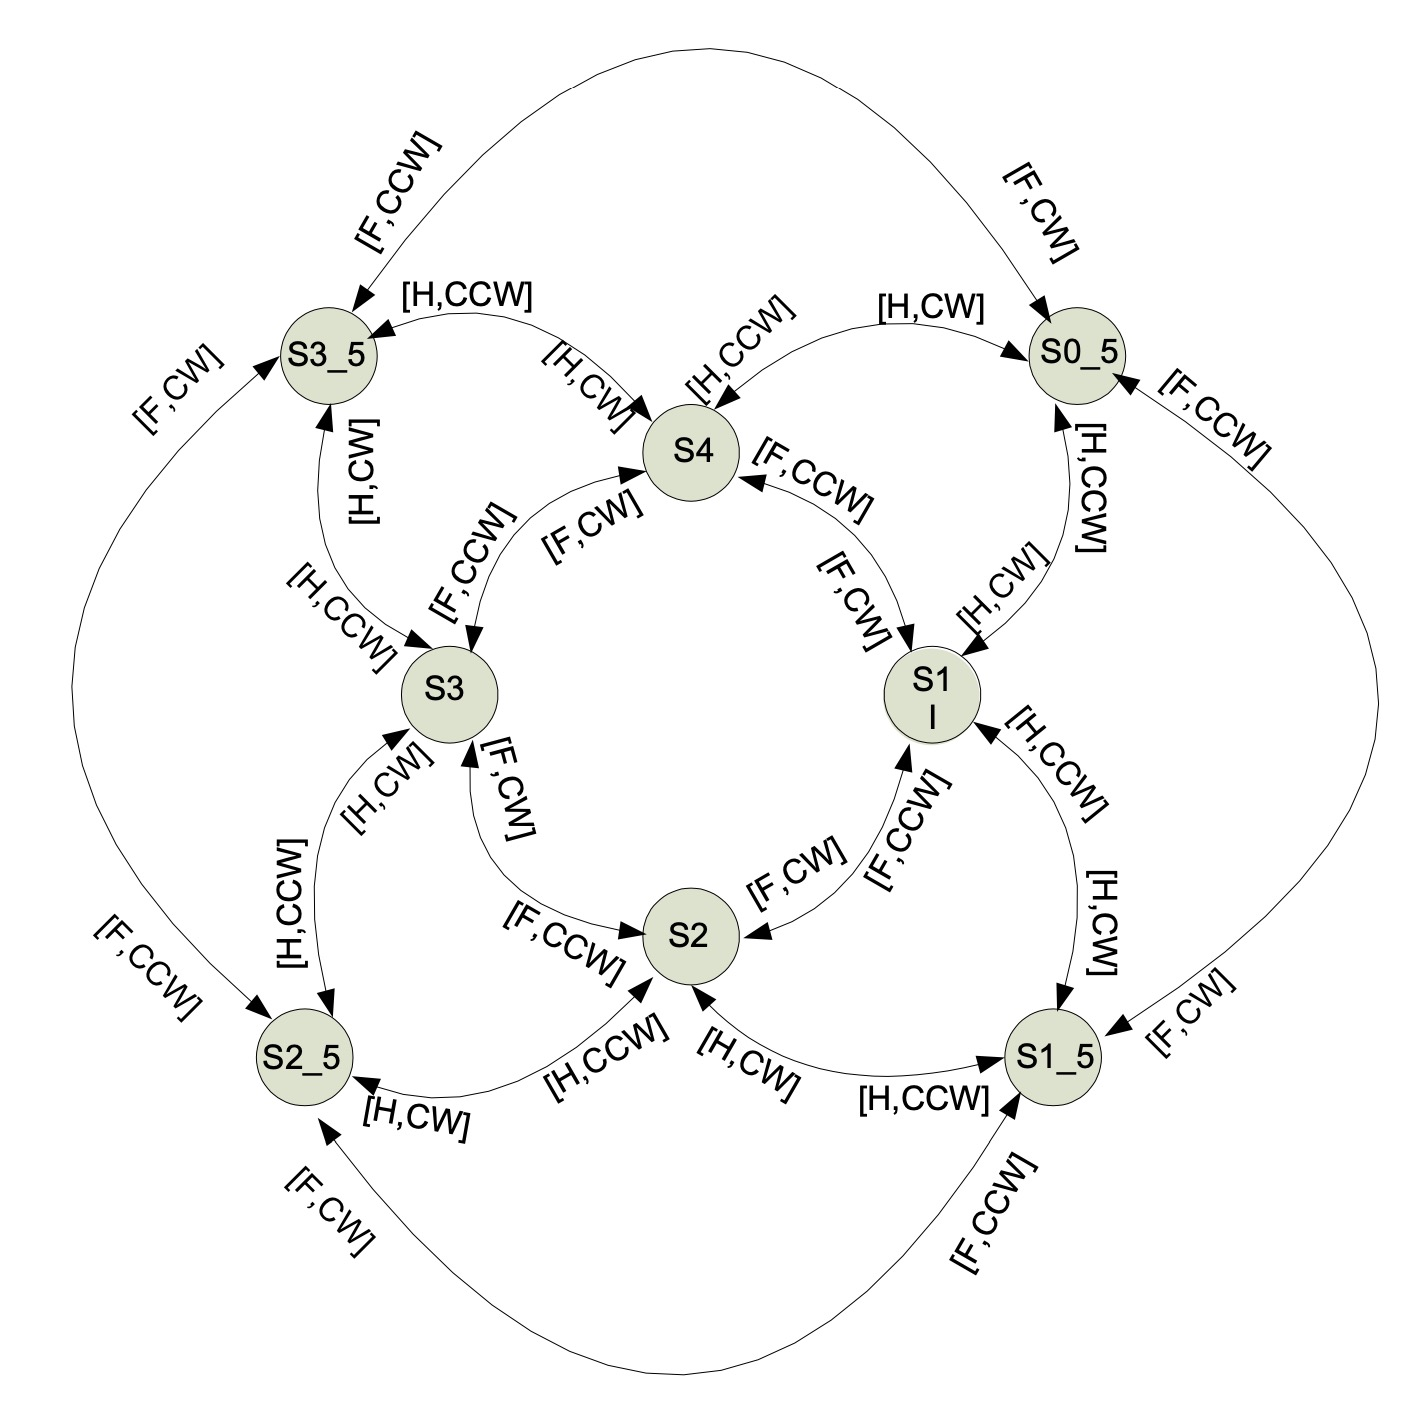
\includegraphics[width=1\textwidth]{FSM}
\caption{FSM Diagram for the Stepper Motor w/ Half and Full Steps}
\end{figure}

Part one, the initializations are shown here:

	\begin{mdframed}[backgroundcolor=code-gray, roundcorner=10pt,
								innerleftmargin=5, innertopmargin=5, innerbottommargin=5]	
	\begin{lstlisting}[language=C, caption=State Machine Initialization, tabsize=2]
	unsigned int stepper_state_machine(
		unsigned int control_mode) {
		enum {S0_5, S1, S1_5, S2, S2_5, S3, S3_5, S4};
		unsigned int return_modes[] = {
			S0_5_HEX, S1_HEX, S1_5_HEX, S2_HEX,
			S2_5_HEX, S3_HEX, S3_5_HEX, S4_HEX
		};
		static int state = S0_5;	// Initialize to 0_5
		...
	\end{lstlisting}
	\end{mdframed}
	
Once again, I used unsigned integers for this function to remain consistent through my program. The \textit{enum} code takes those provided labels (for lack of a better word) and assigns them numbers. This is somewhat equivalent to using macros to define those variables to numbers, but quicker. The reason we do this is to use them in the next segment of code. The state of this machine is then initialized to \textbf{S0\_5} arbitrarily (meaning I could have chosen any state to begin the program on). An import thing to notice here is that the \textbf{state} variable is \textit{static}, meaning that between calls of \textbf{stepper\_state\_machine()}, its value persists. This is extremely important because it removes the need to either pass the current state in as a variable to the function, or have it declared as a global variable. 

The next set of code, \textbf{return\_modes}, is an array of the correct output codes for each state. The important piece of this code is that the order matters. Not only does it logically make sense to have them listed in ascending order, putting them in the same order as the above \textbf{enum} allows for those enumerated labels to index the correct output code. This, along with the state transitions, is shown below:

	\begin{mdframed}[backgroundcolor=code-gray, roundcorner=10pt,
								innerleftmargin=5, innertopmargin=5, innerbottommargin=5]	
	\begin{lstlisting}[language=C, caption=State Machine Transition \& Output Assertion, tabsize=2]
	switch (control_mode) {
		case H_CW:
			state = state-1 < S0_5 ? S4 : state-1;
			break;
		case F_CW:
			state = state-2 < S0_5 ? state+6 : state-2;
			break;
		case H_CCW:
			state = state+1 > S4 ? S0_5 : state+1;
			break;
		case F_CCW:
			state = state+2 > S4 ? state-6 : state+2;
			break;
	}
	return return_modes[state]; // End of function
	\end{lstlisting}
	\end{mdframed}
	
For sake of preserving space, I've only shown one of the eight states. All this very long block of code does is take the \textit{current} state (called \textbf{state}) and then use that, along with the provided \textbf{control\_mode} which is passed as an argument to transition to the next state and assert the correct output. The \textbf{control\_mode} is a return of the previous \textbf{decode\_buttons()} function, and represents what direction and step mode the motor is in. Using the predefined macros of each control mode (\textbf{H\_CW}, \textbf{F\_CW}, etc.) which correspond to their numerical equivalents based off the output of that function, state next state is asserted and it's correct output is given.

The returns of that function are taken and passed to this next section of code, here:

	\begin{mdframed}[backgroundcolor=code-gray, roundcorner=10pt,
								innerleftmargin=5, innertopmargin=5, innerbottommargin=5]	
	\begin{lstlisting}[language=C, caption=Applying Output to the Motor's Pins, tabsize=2]
	void output_to_stepper_motor(unsigned int hexcode) {
		unsigned int output = hexcode << 7;
		unsigned int current = PORTB & (BIT_7 | BIT_8
			| BIT_9 | BIT_10);

		PORTClearBits(IOPORT_B, ~current & output);
		PORTSetBits(IOPORT_B, output);
	}
	\end{lstlisting}
	\end{mdframed}
	
Using the current state's necessary output (as detailed in the lab document), this function first shifts those four bits so they line up one pins 7 through 10 (hence the bit-shift), and then asserts them on \textbf{PORTB}. I first encountered the problem where the old state's output wouldn't be overwritten, leading to all bits being high after a few transitions), so I clear those pins at first to avoid this problem. In order to prevent some bits that need to stay high between transitions from quickly turning on and then off, the current state of the motor's output is looked at, and then only the bits that are currently 1 and becoming 0's are turned off.

The final, non-main, function written for this lab was \textbf{sw\_delay()}. This is shown in Listing 9, and delays the correct amount of time to generate the correct rotational speed on the motor.

	\begin{mdframed}[backgroundcolor=code-gray, roundcorner=10pt,
								innerleftmargin=5, innertopmargin=5, innerbottommargin=5]	
	\begin{lstlisting}[language=C, caption=Motor Delay Code, tabsize=2]
	void sw_delay(unsigned int rpm, unsigned int
		control_mode, unsigned int hexcode) {
		unsigned int delay = (control_mode & 0x01) ?
			(60000 / (rpm * 100)) : (60000 / (rpm * 200));

		output_to_stepper_motor(hexcode);
		LATBINV = LEDC;
		delayMS(delay);

		LATBINV = LEDB;
	}
	\end{lstlisting}
	\end{mdframed}
	
The first line, the \textbf{delay} calculation, implements the following formula provided by the lab handout:

$$T_{delay} (ms)=\frac{60000}{X * 100 * MODE}$$

Where X is the desired RPM of the motor, and MODE is either 1 or 2 for full-step and half-step mode respectively.

So all this does is calculate the necessary delay by seeing if the provided \textbf{control\_mode} is in full or half-step mode, and then using the variable RPM. Although we are currently using a fixed RPM of 15, it was trivial to add in a variable for it, which might be useful later.

The provided output code is sent to the motor (through a function call of Listing 8), and then the previously calculated amount of time is waited. The \textbf{delayMS()} function is not shown here as it is identical to last lab's implementation. The reason for toggling the LED's is to see how long the non-waiting code takes (that's what \textbf{LEDC} is for) and to see how often the motor is pulsed (with \textbf{LEDB}).

At this point, the only code left to write was the program's infinite loop that calls all of these functions. Since the \textbf{sw\_delay()} function takes care of all the waiting, this is a very simple block of code.

	\begin{mdframed}[backgroundcolor=code-gray, roundcorner=10pt,
								innerleftmargin=5, innertopmargin=5, innerbottommargin=5]	
	\begin{lstlisting}[language=C, caption=Infinite Program Loop, tabsize=2]
	int main() {
		system_init();
		unsigned int button_status = 0;
		unsigned int control_mode  = 0;
		unsigned int motor_hexcode = 0;
	
		while (1) {
			LATBINV = LEDC;
			button_status = read_buttons();	
			control_mode  = decode_buttons(button_status);
			motor_hexcode = stepper_state_machine(control_mode);
			sw_delay(RPM, control_mode, motor_hexcode);	
		}
		return 0;
	}
	\end{lstlisting}
	\end{mdframed}
	
This is all quite trivial, the only thing of interest is the toggle of \textbf{LEDC} at the beginning of the loop. This is, as discussed before, useful for seeing how long the non-delayed code takes.

\section{Testing and Validation}
\begin{table}[h]
\centering
\begin{tabular}{cc|ccc}
\multicolumn{2}{c|}{\textbf{Inputs}} & \multicolumn{3}{c}{\textbf{Stepper Parameters}} \\
\hline
BTN2 & BTN1 & Step Mode & Desired Step Delay & Measured Step Delay \\
\hline
Off & Off & FS &  40ms & 40.000ms \\
Off & On & HS & 20ms & 20.000ms \\
On & Off & HS & 20ms & 20.100ms \\
On & On & FS & 40ms & 39.800ms \\
\end{tabular}
\caption{Delay accuracy in different modes}
\end{table}
The screen-captures from the Oscilloscope are attached in Section 6.

I toggled one of the unused LED's (\textbf{LEDC}) on port G and then hooked up the oscilloscope to that LED output. The LED was set to toggle at the beginning of the \textbf{while(1)} loop (as seen in Listing 10), and then turn off at just before the \textbf{delayMS()} function was called (shown in Listing 9). Once a pulse was captured on this line, I measured how long it was high, and obtained 2.9 $\mu$s as the time it took to execute the non-delayed code.

\section{Questions}
\begin{enumerate}
\item A very popular method of implementing an FSM in C is to use function pointers. By creating a pointer that can be pointed an arbitrary function, that pointer can execute different arbitrary functions, and can be used to represent different states in the FSM. This implementation can be really useful for round-robin style tasks, or FSM's that need more complicated states, more than you'd ideally put in a huge conditional statement. The downside of this type of implementation is that it requires quite a bit of overhead (a lot of functions depending on the project), and can be somewhat difficult to follow.

An FSM can also be implemented using \textit{goto} to move between modes. In this case, the code would have been like: \textit{goto S0\_5 ... S0\_5: do { ... } while(... ), etc.} The downside of this is that the code has to be laid out somewhat linearly, and it does not take advantage of many higher-level C features. The upside is the relative simplicity and how flexible it is.\footnote{https://rosettacode.org/wiki/Finite\_state\_machine}

The final method, and my personal favorite, is what we used here in this lab. I like the ease of understanding that the large conditional statement provides. I also believe it is quite easy to debug and add onto (should the need arise). The downside is how bloated the statement can become, especially with more complicated FSMs, and it is not exactly elegant.

\item The biggest difference between an FSM on a FPGA and a micro-controller is that the FPGA can process instructions concurrently, due to the physical nature of their construction. This means that very time-sensitive interrupts (like the button press, in this example) could be triggered immediately, as opposed to the sequential nature of the micro-controller's processing.\footnote{https://www.7pcb.com/blog/fpgas-and-microcontrollers.php}

\item The buttons are presently sampled every 20-40ms, depending on the mode (before the motor is delayed each loop). At this current delay, it is \textit{very} unlikely to have any consequences for this kind of application. But, if I were to hypothetically pressed the button during the delay period of the code, and then release it before the \textbf{read\_buttons()} function was called, that press would be completely ignored and the stepper motor would not change its status at all. One solution to this that comes to mind is to implement a non-blocking function in \textbf{delayMS()} so that the buttons can be read as often as possibly by the infinite loop. Another possibility is to have the button presses trigger an interrupt.
\end{enumerate}

\section{Conclusion}
This lab demonstrated many important aspects of using a micro-controller, especially regarding real-world circumstances where timing is important. This lab really highlighted the limitations of timing on a micro-controller (at least with how we're doing it). Specifically, being 'blocked' out of sampling the buttons while we're waiting to send the next pulse to the motor is a \textit{huge} problem with regards to missing inputs (especially for similar, more time-sensitive inputs). That, combined with the fact that the current delay function we're using has limited delay capability really showcases the problem with more expansive timing functionality on a micro-controller.

On the other hand, the implementation of a finite state machine went very well. Transitioning between states was very clear to understand and implement, and the use of static variables makes this type of program easy to expand. Luckily this particular FSM was very circular in its nature, so the implementation was even easier than a normal one (which would require a long series of conditionals statements).

\newpage
\section{Attachments}
\begin{figure}[htb]
\centering
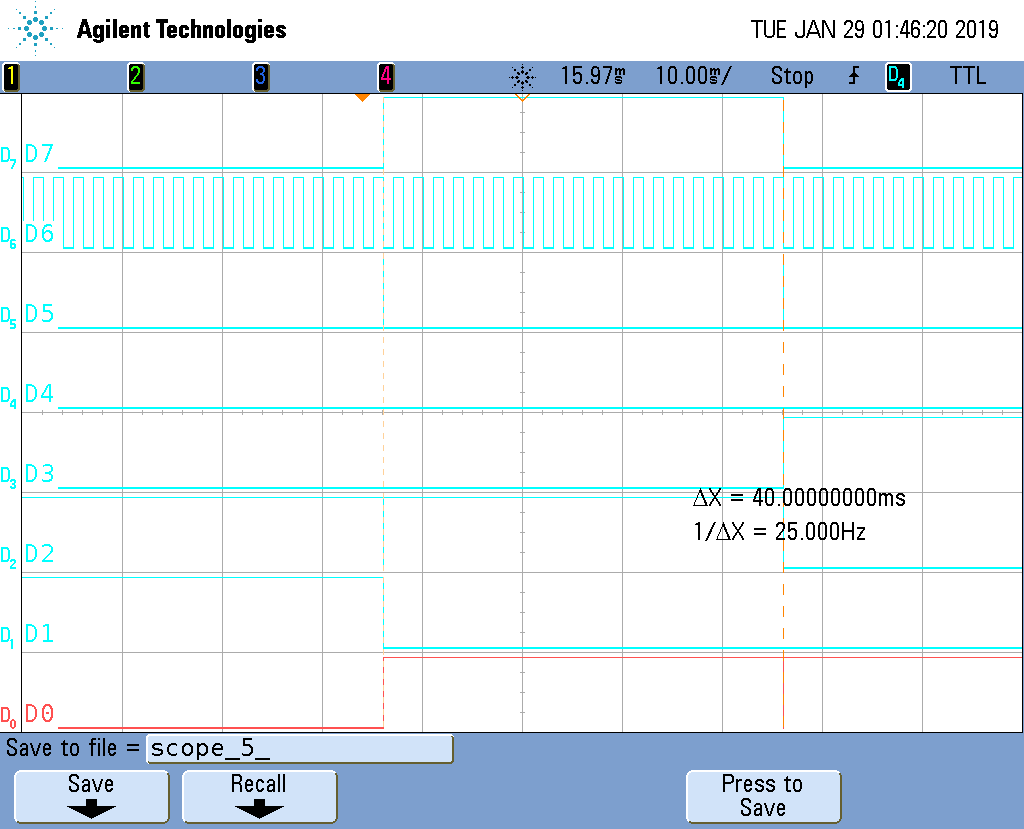
\includegraphics[width=.8\textwidth]{0-0.png}
\caption{The off-off 40ms delay}
\end{figure}

\begin{figure}[htp]
\centering
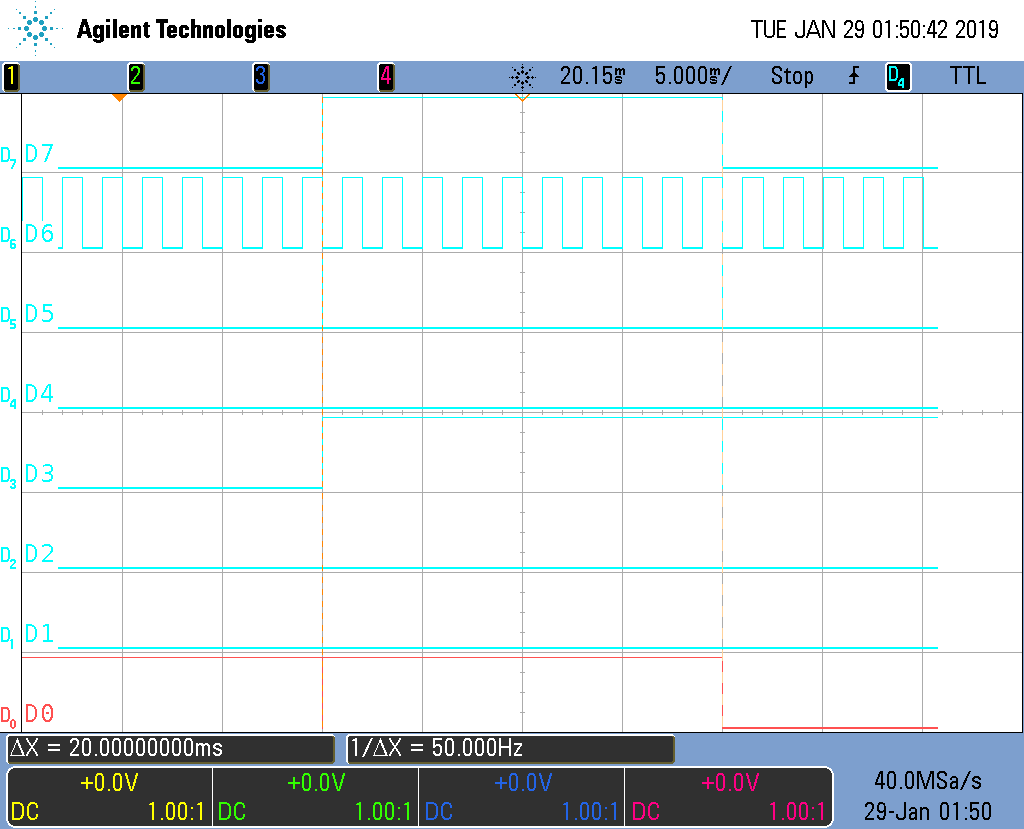
\includegraphics[width=.8\textwidth]{0-1.png}
\caption{The off-on 20ms delay}
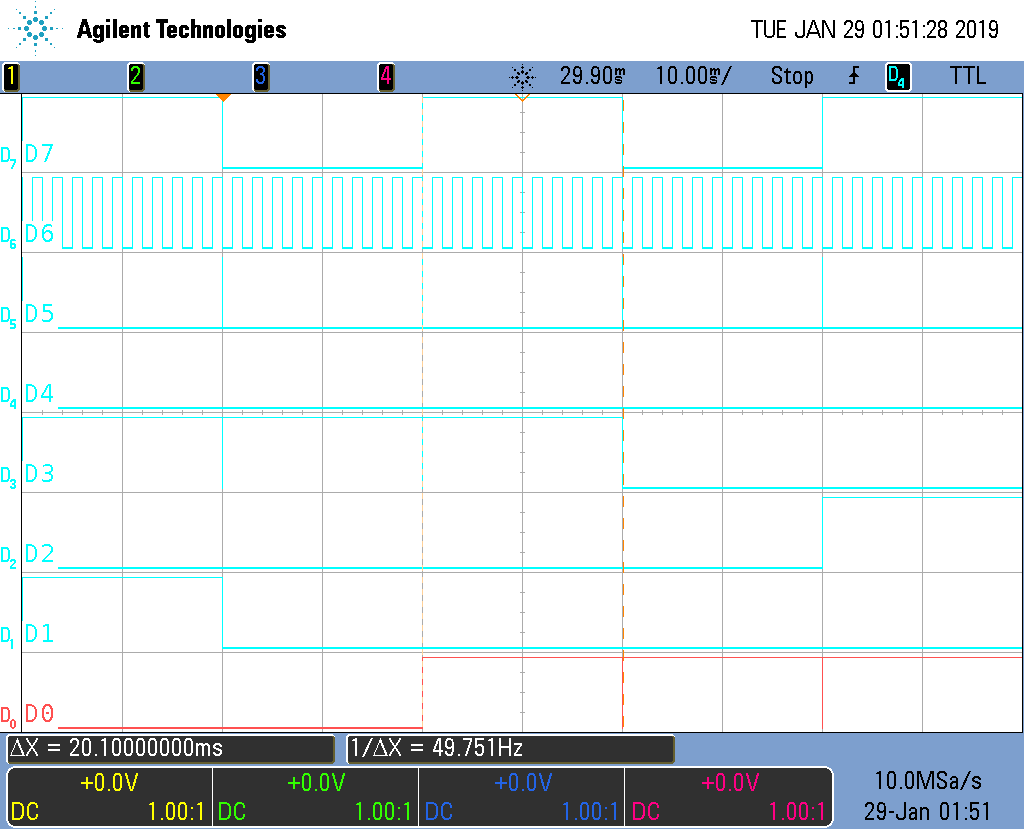
\includegraphics[width=.8\textwidth]{1-0.png}
\caption{The on-off 20ms delay}
\end{figure}

\begin{figure}[htb]
\centering
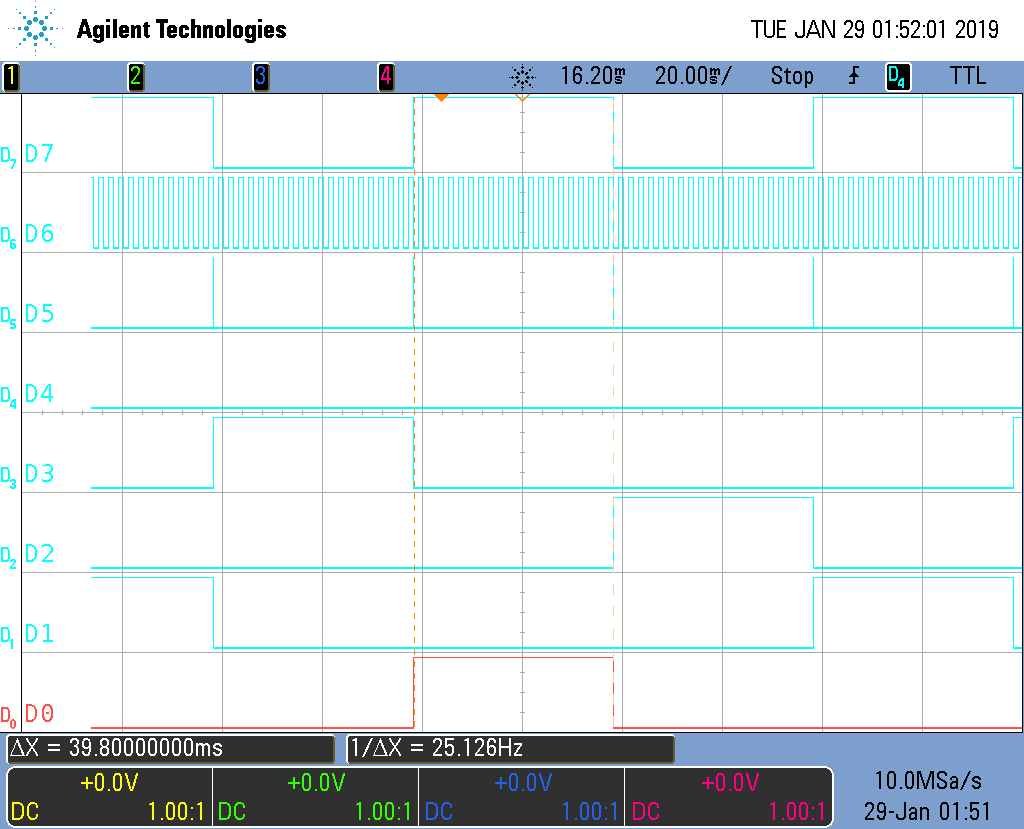
\includegraphics[width=.8\textwidth]{1-1.png}
\caption{The on-on 40ms delay}
\end{figure}

\end{document}